\subsection*{ГЛ9 1}
\textbf{a)}\\
Пусть $\Phi$ -- некая фигура, ее грани это пересечения замкнутой фигуры с ее опорной гиперплоскостью, вершины -- нульмерные грани. То есть если касательная проведенная из некой точки $a \in \Phi$ к $\Phi$ в пересечении с $\Phi$ содержит только $a$, то точка $a$ является вершиной.
\begin{figure}[h!]
	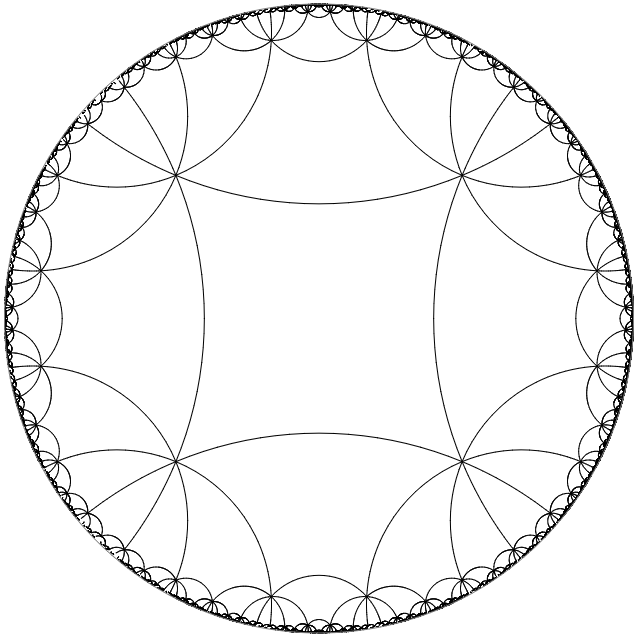
\includegraphics[width=0.5\linewidth]{pic12}
\end{figure}\\
У фигуры на картинке вершинами являются $\Phi\backslash [A, B] \cup [C, D] = (C, A) \cup (B, D)$ -- 2 полуокружности с выколотыми точками. Объединение двух открытых множеств -- открытое множество, откуда следует что выпуклое множество удовлетворяет условию.\\


\vskip 0.3in
\noindent
\textbf{б)}\\
Рассмотрим фигуру $\Phi \in \mathbb{R}^3$. Она образована движением параболы с вершиной $O$ вдоль оси $AB$, причем ширина параболы менялась во время движения по $AB$ так как показано на рисунке (чтобы $CME$ и $DKF$ были выпуклыми). Таким образом, имеется замкнутая выпуклая фигура $\Phi$, ее граница --
$X$ $\cup$ четырехугольник $CDFE$ $\cup$ отрезок $AB$.\\
\begin{figure}[h]
	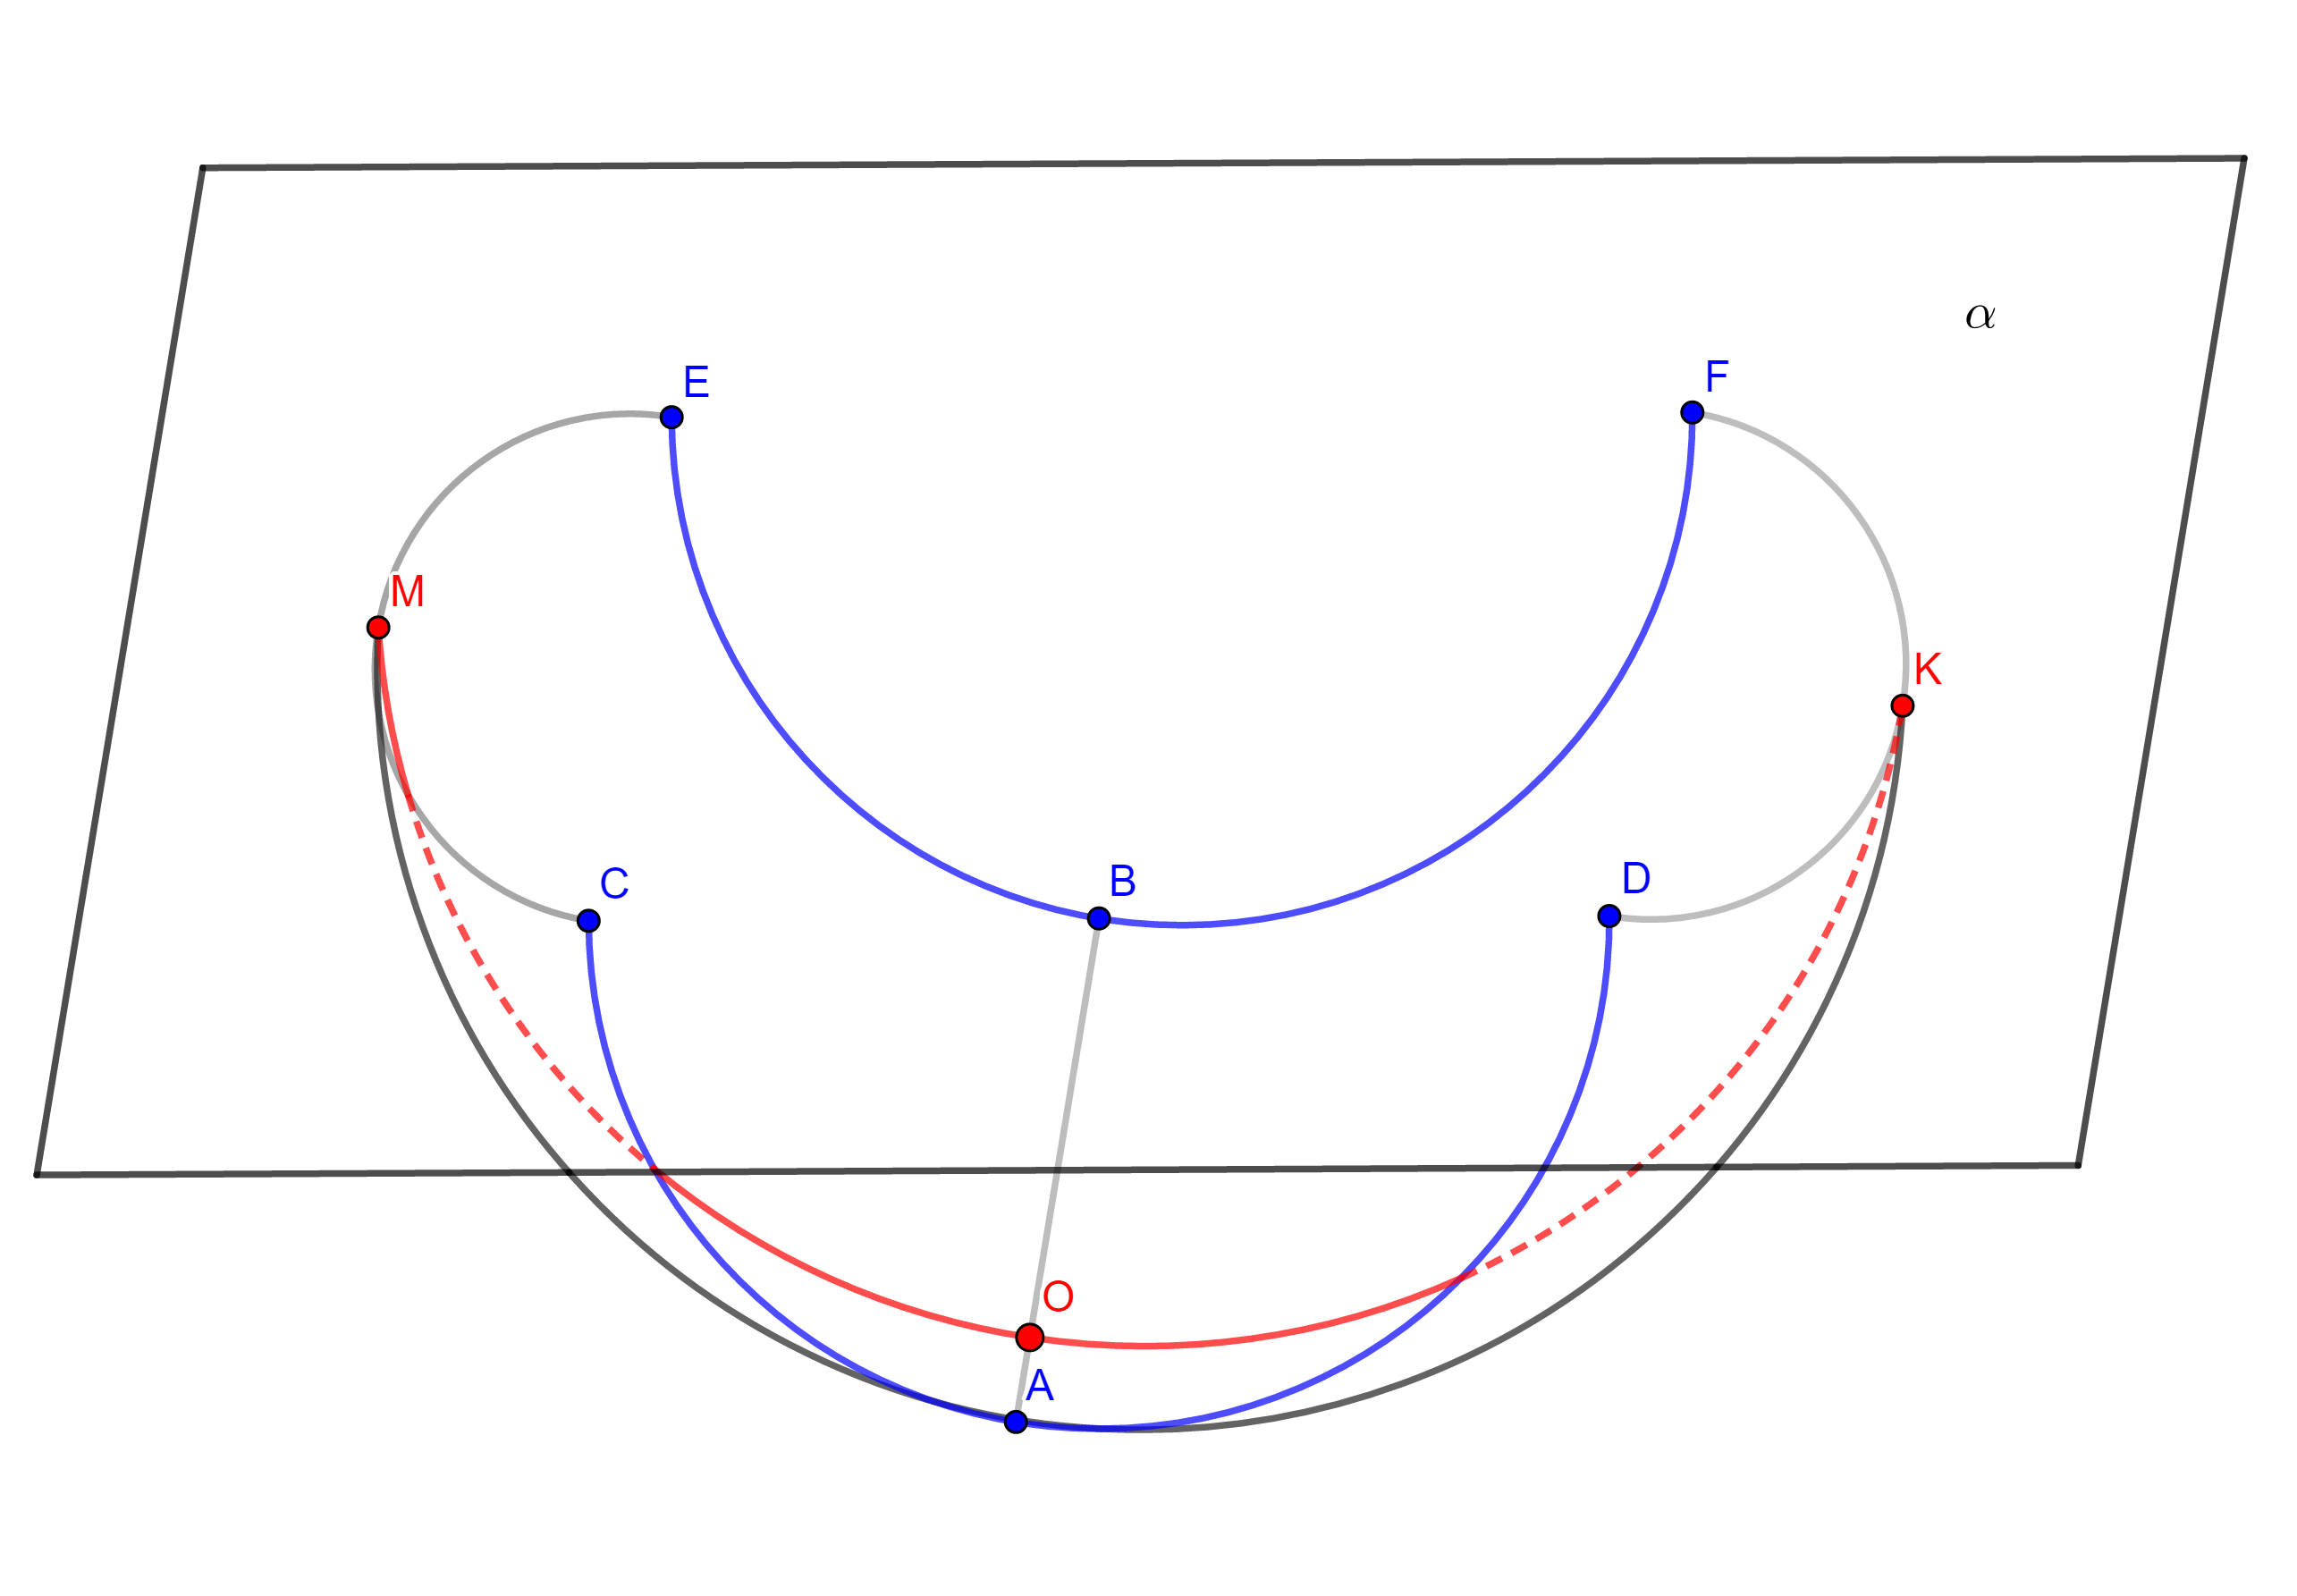
\includegraphics[width=0.5\linewidth]{pic21}
\end{figure}\\
По определению, крайней точкой фигуры $\Phi$ называется точка, которая не является внутренней точкой никакого отрезка $[a,b] \in \Phi$.\\
У параболы с вершиной $A$ крайними точками являются все точки, кроме $A, C, D$, следовательно, множество крайних точек не замкнуто, тк существует предельная точка $A$, не лежащая во множестве крайних точек.\\
Заметим, что это множество не только не замкнуто, но и открыто, тк оно гомеоморфно объединению 2х интервалов. Объединение бесконечного числа открытых множеств -- открыто.\\
Таким образом, крайней точкой фигуры $\Phi$ является объединение бесконечного числа незамкнутых множеств -- незамкнутое множество $X \slash (CE \cup DF \cup AB)$\\